\documentclass[titlepage, twoside, a4paper, 12pt]{article}
\usepackage[swedish]{babel}
\usepackage[utf8]{inputenc}
\usepackage{verbatim}
\usepackage{fancyhdr}
\usepackage{graphicx}
\usepackage{parskip}
% Include pdf with multiple pages ex \includepdf[pages=-, nup=2x2]{filename.pdf}
\usepackage[final]{pdfpages}
% Place figures where they should be
\usepackage{float}

% Float for text
\floatstyle{ruled}
\newfloat{program}{thp}{lop}
\floatname{program}{RSSxml}


% vars
\def\title{RSS}
\def\preTitle{Laboration 2}
\def\kurs{Applikationsprogrammering i Java, HT-08}

\def\namn{Anton Johansson}
\def\mail{dit06ajn@cs.umu.se}
 \def\pathtocode{$\sim$dit06ajn/edu/apjava/lab2}

\def\handledareEtt{Johan Eliasson, johane@cs.umu.se}
\def\handledareTva{Tor Sterner-Johansson, tors@cs.umu.se}
\def\handledareTre{Daniel Henriksson, danielh@cs.umu.se}

\def\inst{datavetenskap}
\def\dokumentTyp{Laborationsrapport}

\begin{document}
\begin{titlepage}
  \thispagestyle{empty}
  \begin{small}
    \begin{tabular}{@{}p{\textwidth}@{}}
      UMEÅ UNIVERSITET \hfill \today \\
      Institutionen för \inst \\
      \dokumentTyp \\
    \end{tabular}
  \end{small}
  \vspace{10mm}
  \begin{center}
    \LARGE{\preTitle} \\
    \huge{\textbf{\kurs}} \\
    \vspace{10mm}
    \LARGE{\title} \\
    \vspace{15mm}
    \begin{large}
        \namn, \mail \\
        \texttt{\pathtocode}
    \end{large}
    \vfill
    \large{\textbf{Handledare}}\\
    \mbox{\large{\handledareEtt}}
    \mbox{\large{\handledareTva}}
    \mbox{\large{\handledareTre}}
  \end{center}
\end{titlepage}

\newpage
\mbox{}
\vspace{70mm}
\begin{center}
\textit{Till Cecilia...}
\end{center}
\thispagestyle{empty}
\newpage

\pagestyle{fancy}
\rhead{\today}
\lhead{\namn, \mail}
\chead{}
\lfoot{}
\cfoot{}
\rfoot{}

\tableofcontents
\cleardoublepage

\rfoot{\thepage}
\pagenumbering{arabic}

\section{Problemspecifikation}\label{Problemspecifikation}
% Beskriv med egna ord vad uppgiften gick ut på. Är det någonting som
% varit oklart och ni gjort egna tolkningar så beskriv dessa.
Denna laboration gick ut på att skriva en RSS-läsare med grafiskt
användar\-gränssnitt i programmerings\-språket Java. RSS står för
Really Simple Syndication och är ett filformat som används för att på
ett standardiserat sätt spara undan information i en lista. Oftast
består denna information av något typ av artikel.

En RSS-läsare fungerar ungefär som en mailklient, det vill säga
användare kan välja att prenumerera på valda RSS-flöden. Läsaren visar
upp artiklarna som finns i RSS-flödet, dessa kan läsas och markeras då
oftast som lästa på något sätt.

Exempel på RSS-flöde:\\
\verb!http://sydsvenskan.se/senastenytt/?context=senasteNyttRss!

Problemspecifikation finns i original på:\\
\verb!http://www.cs.umu.se/kurser/5DV085/HT08/labbar/lab2.html!

\section{Användarhandledning}\label{Anvandarhandledning}
% Förklara var programmet och källkoden ligger samt hur man startar,
% kompilerar och använder det.
Programmet ligger i katalogen:\\
\texttt{\pathtocode}

Från denna katalog kompileras programmet med kommandot:

\verb!salt:~/edu/apjava/lab2> ant!

De kompilerade filerna hamnar i underkatalogen \verb!bin!. Från denna
katalog körs programmet med kommandot

\verb!salt:~/edu/apjava/lab2/bin> java -cp .:../lib/jdom.jar JeedReader!

Alternativt kan programmet köras direkt från huvudmappen med
kommandot:

\verb!salt:~/edu/apjava/lab2> ant test-run!

När programmet startar läses föregående sparade flöden från katalogen
\verb!bin/config! in. Är det första gången programmet startar kommer
denna katalog att vara tom. Finns det flöden i katalogen kommer
gränssnittet att se ut ungefär som i figur \ref{fig:gui-out}.

\begin{figure}[H]
  \begin{center}
    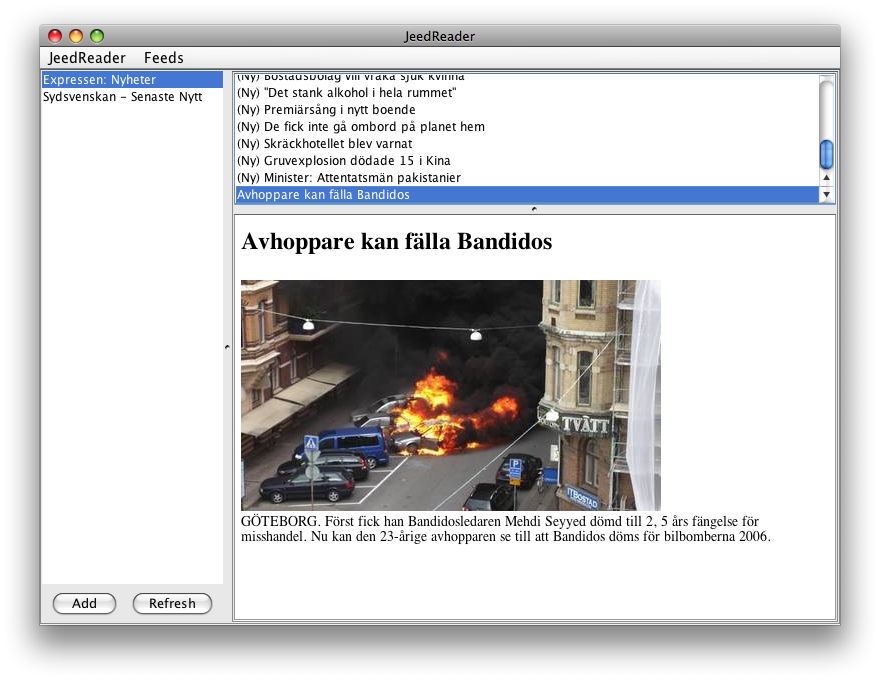
\includegraphics[width=110mm]{images/gui-out.png}
    \caption{Användargränssnitt.}
    \label{fig:gui-out}
  \end{center}
\end{figure}

Gränssnittet består av en lista till vänster som innehåller flöden
användaren lagt till, ovan till höger visas titeln för varje artikel i
valt flöde och under visas beskrivningen av vald artikel.

När en artikel är vald markeras denna som läst genom att texten
\verb!(Ny)! försvinner från dess titel i listan. Det går att lägga
till nya flöden via knappen \textit{Add} eller via menyn
\textit{Feeds/Add feed}.

För att uppdatera alla flöden används knappen \textit{Refresh} eller
menyvalet \textit{Feeds} och sedan \texttt{Update~all~feeds}. För att
enbart uppdatera markerat flöde används menyvalet
\textit{Feeds/Update~selected~feed}, varje flöde uppdateras även varje
gång de markeras i listan.

Källkoden ligger i underkatalogen \verb!src!.

\section{Systembeskrivning}\label{Systembeskrivning}
% Beskriv översiktligt hur programmet är uppbyggt och hur det löser
% problemet.
Programmet är uppbyggt enligt \textit{Model-View-Controller}
modell. De tre huvudklasserna som driver programmet består av
\textit{JeedReader} som motsvarar programmets \textit{Controller}-del,
\textit{JeedView} som motsvarar \textit{View}-delen och
\textit{JeedModel} som motsvarar \textit{Model}-delen. Utöver dessa
finns även ett antal klasser som har hand om mer specifikt beteende,
främst är dessa klasser till hjälp för klassen
\textit{JeedReader}. Klassdiagram finns i figur~\ref{fig:classUML}.

\subsection{API}
API-dokumentation finns på sidan:\\
\verb!http://www.cs.umu.se/~dit06ajn/apjava/lab2/!

\newpage
\begin{figure}[H]
  \begin{center}
    \makebox[0cm]{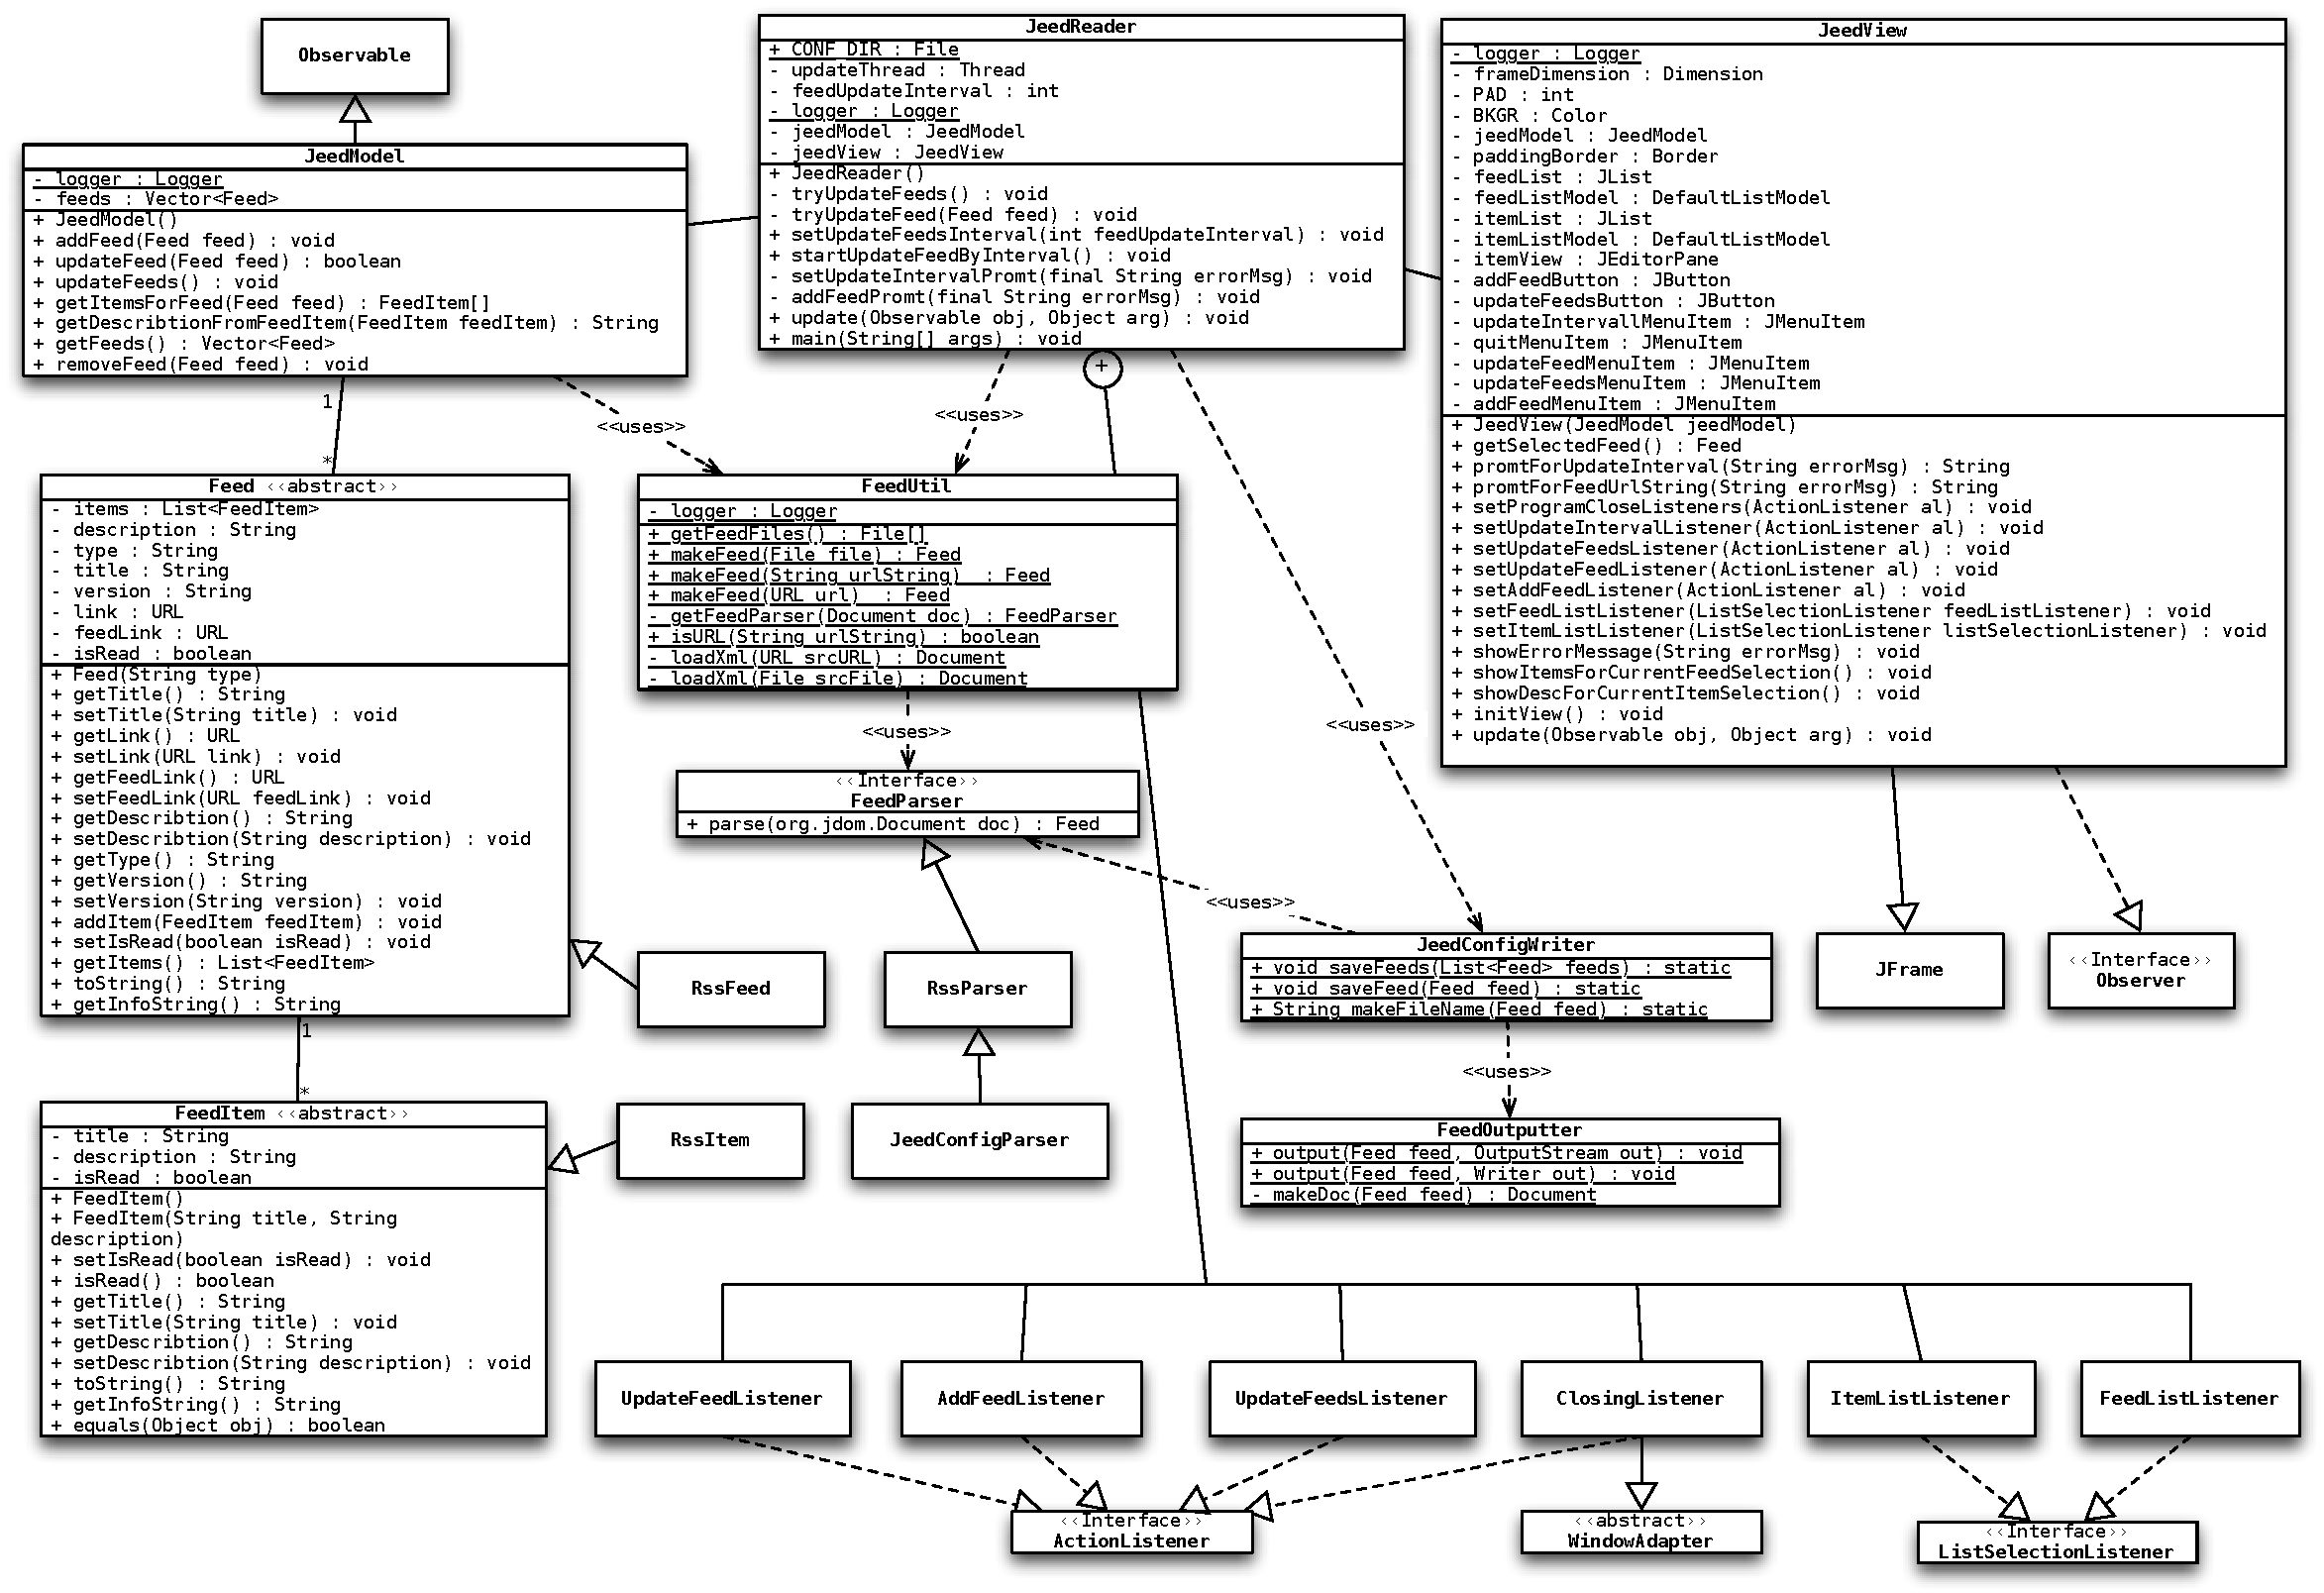
\includegraphics[width=230mm,angle=90]{images/classUML.pdf}}
    \caption{Klassdiagram.}
    \label{fig:classUML}
  \end{center}
\end{figure}

\subsection{JeedReader.java}\label{JeedReader}
Klassen \textit{JeedReader} är programmets huvudklass, med denna klass
startas programmet. I \textit{Model-View-Controller}-modellen så
motsvarar denna klass \textit{Controllern}, det vill säga klassen
ansvarar för att bygga upp programmet och hantera användares
handlingar. \textit{JeedReader}s konstruktor gör följande:

\begin{itemize}
\item Skapar en \textit{JeedModel} och skickar med denna instans till
  konstruktorn i \textit{JeedView}.

\item Flöden för alla filer, som fås av metoden
  \textit{FeedUtil.getFeedFiles()}, se sektion \ref{getFeedFiles()},
  skapas och läggs till i instansen av \textit{JeedModel}.

\item Inre klasser som implementerar olika typer av
  \textit{EventListener}s instansernas och fästs vid olika komponenter
  i \textit{JeedView} genom ''set''-metoder i \textit{JeedView}.

\item Klassen \textit{JeedView} läggs till som \textit{Observer} till
  klassen \textit{JeedModel}. Detta för att kunna meddela
  \textit{JeedView} varje gång något ändras i \textit{JeedModel} som
  bör påverka det grafiska gränssnittet.

\item Startar en tråd som uppdaterar alla flöden vid bestämt
  intervall.
  
\item \textit{JeedView} visas för användaren.
\end{itemize}

Klassen \textit{JeedReader} sätts även som lyssnare
(\textit{Observer}) till klassen \textit{JeedModel}, varje gång
uppdatering sker i \textit{JeedModel} sparas konfigurationsfilerna,
innehållande information om flödena, i katalogen \textit{config}.

Källkod finns i bilaga \ref{JeedReader.java}.

\subsection{JeedView.java}\label{JeedView}
Klassen \textit{JeedView} representerar programmets grafiska
gränssnitt. Alla grafiska komponenter skapas och metoder för att visa
upp dialog- och felrutor deklareras.

Metoder för att fästa olika typer av \textit{EventListener}s vid
specifika komponenter såsom knappar, listor och menykomponenter
deklareras.

Klassen implementerar gränssnittet \textit{Observer} för att kunna
lyssna på uppdateringar som kommer från \textit{JeedModel}. Dessa
uppdateringar fångas i metoden \textit{update(Observable obj, Object
  arg)}. Första parametern till \textit{update} tar emot objekt, av
typen \textit{Observable}, i detta program kommer detta objekt att
vara programmets instans av \textit{JeedModel}. Andra parametern är
ett valbart objekt som indikerar på vad som har ändrats i
\textit{JeedModel}. % TODO hur

Källkod finns i bilaga \ref{JeedView.java}.

\subsection{JeedModel.java}\label{JeedModel}
Klassen \textit{JeedModel} är en representation av programmets
data. Här sparas alla flöden och metoder för att hämta, lägga till och
ta bort flöden är implementerade. Klassen utökar
\textit{java.util.Observable} och meddelar alla klasser som
registrerat sig som intressenter för denna klass när ändringar i
\textit{JeedModel}.

Flöden som användare lägger till i programmet sparas i \textit{Feed}
referenser, den bakomliggande implementationen är dock i denna
implementation enbart av typen \textit{RssFeed}.

% TODO ändringar per flöde, skicka med flödet som argument

Källkod finns i bilaga \ref{JeedModel.java}.

\subsection{JeedConfigParser.java}\label{JeedConfigParser}
Klassen \textit{JeedConfigParser} utökar klassen \textit{RssParser}
och överlagrar dess metoder \textit{parse(org.jdom.Document)} och
\textit{parseItem(org.jdom.Element, RssItem)}. Denna utökade
funktionalitet av \textit{RssParser} hanterar dokument som är sparade
av själva programmet. Dessa dokument har en \textit{jss}-tag som root-element
artiklar med ett attribut \textit{isRead}. Metoden
\textit{parse(org.jdom.Document)} returnerar en instans av
\textit{RssFeed}, se sektion \ref{RssFeed}.

Källkod finns i bilaga \ref{JeedConfigParser.java}.

\subsection{Feed.java}\label{Feed}
Den abstrakta klassen \textit{Feed} implementerar alla funktioner som
bör vara gemensamma för alla typer av flöden som ska kunna sparas i
programmet. Främst är ''Get''- och ''Set''-metoder implementerade för
information som rör flöden. Exempel på sådan information är flödets
titel, URL, typ, version, beskrivning.

Metoden \textit{toString()} är överlagrad för att returnera flödets
titel. Detta används i det grafiska gränssnittet för att skriva ut
flöden i en lista.

Källkod finns i bilaga \ref{Feed.java}.

\subsection{FeedItem.java}\label{FeedItem}
Den abstrakta klassen \textit{FeedItem} implementerade alla funktioner
som bör vara gemensamma för flödens artiklar. Främst är ''Get''- och
''Set''-metoder implementerade för information som rör
artiklar. Exempel på sådan information är artiklars titel,
beskrivning, om artikeln är läst eller ej.

Metoden \textit{toString()} är överlagrad för att returnera artikelns
status, det vill säga om den är läst eller ej och dess titel. En läst
artikel får strängen \textit{(Ny)} insatt före dess titel. Detta
används i det grafiska gränssnittet för att skriva ut artiklar i en
lista.

Källkod finns i bilaga \ref{FeedItem.java}.


\subsection{JeedConfigWriter.java}\label{JeedConfigWriter}
Klassen \textit{JeedConfigWriter} använder sig av klassen
\textit{FeedOutputter}, för att spara en eller flera flöden som filer
i katalogen som definieras av konstanten \textit{CONF\_DIR} i klassen
\textit{JeedReader}. Filnamnen som sparas bestäms av flödenas
\textit{URL}, och kommer därför alltid att bli unika för varje flöde.

Källkod finns i bilaga \ref{JeedConfigWriter.java}.

\subsection{FeedOutputter.java}\label{FeedOutputter}
Klassen \textit{FeedOutputter} skriver ut flöden, \ref{Feed}, till
antingen en instans av \textit{java.io.OutputStream} eller en instans
av \textit{java.io.Writer}. I ett mellanled skapas tillfälligt en
instans av typen \textit{org.jdom.Document}, det är informationen i
detta objekt som sedan skrivs ut. I nuläget hämtas inte all
information ur flödet, se begränsningar sektion
\ref{Begransningar}. % TODO

När flödena sparas undan till disk ändras root-taggen från
\textit{rss} till \textit{jss} och ett attribut, \textit{feedLink},
sätts till flödets URL. Varje artikel i flödet får även ett attribut
\textit{isRead} som skriver ut artikelns, \textit{FeedItem}, fält
\textit{isRead}.

Källkod finns i bilaga \ref{FeedOutputter.java}.

\subsection{FeedParser.java}\label{FeedParser}
\textit{FeedParser} är ett gränssnitt som alla parsers i programmet
ska implementera. Gränssnittet innehåller en metod
\textit{parse(org.jdom.Document)} som returnerar ett flöde av typen
\textit{Feed}.

Källkod finns i bilaga \ref{FeedParser.java}.

\subsection{FeedUtil.java}\label{FeedUtil}
Klassen \textit{FeedUtil} innehåller enbart statiska
''hjälp\-metoder'' för resten av programmet. Metoder för att skapa
flöden från textsträngar eller av \textit{java.net.URL} är
implementerade.

Metoden \textit{getFeedFiles()}\label{getFeedFiles()} returnerar alla
flödes-filer som programmet sparar sina flöden i. Dessa filer ligger i
katalogen \textit{config}, bestämd av konstanten \textit{CONF\_DIR} i
klassen \textit{JeedReader}, och har filnamn som slutar med
\verb!feed.xml!.

Metoden \textit{getFeedParser(org.jdom.Document)} används internt i
klassen för att returnera en korrekt implementation av gränssnittet
\textit{FeedParser}. I nuläget returneras en instans av
\textit{RssParser}, se sektion \ref{RssParser}, om root-elementet i
det inskickade dokumentet är en \textit{rss}-tag och dess attribut
\textit{version} består av strängen ''2.0''. Om det inskickade
dokumentets root-element är en \textit{jss}-tag retureras en instans
av \textit{JeedConfigParser}, se sektion \ref{JeedConfigParser}.

Källkod finns i bilaga \ref{FeedUtil.java}.

\subsection{RssFeed.java}\label{RssFeed}
Klassen \textit{RssFeed} utökar den abstrakta klassen
\textit{Feed}. \textit{RssFeed} inför ytterligare fält, ''get''- och
''set''-metoder som enbart gäller för flöden av typen RSS. I denna
implementation är enbart version 2.0 av RSS accepterade, dock kan
ytterligare funktionalitet implementeras i denna klass eller som
underklasser till \textit{RssFeed} eller \textit{Feed}.

Källkod finns i bilaga \ref{RssFeed.java}.
\subsection{RssItem.java}\label{RssItem}
Klassen \textit{RssItem} utökar den abstrakta klassen
\textit{FeedItem}. Ytterligare fält och metoder kan implementeras i
denna klass för att hantera ''RSS 2.0''-taggar.

Källkod finns i bilaga \ref{RssItem.java}.
\subsection{RssParser.java}\label{RssParser}
Klassen \textit{RssParser} implementerar gränssnittet
\textit{FeedParser}. Metoden \textit{parse(org.jdom.Document doc)}
sköter tolkningen av dokumentet medskickat i parametern och returnerar
en \textit{RssFeed}. Taggar ur specifikation för RSS 2.0 tolkas och
sparas undan i en ny instans av \textit{RssFeed}.

Källkod finns i bilaga \ref{RssParser.java}.
\subsection{config}
I katalogen \textit{config} sparas alla flöden undan av
programmet. Flöden får filnamn bestående av länken till flödet och
avslutas med \verb!feed.xml!.

\section{Begränsningar}\label{Begransningar}
% Vilka problem och begränsningar har din lösning av uppgiften? Hur
% skulle de kunna rättas till?

Programmet får ses som början av implementation av en fullt fungerande
RSS-läsare. Hantering av artiklars alla godkända taggar är ej
gjord. Enbart titel och beskrivning används och även där hade det
behövts göras mer felkontroller för att vara säker på att de
finns. Enligt specifikationen av RSS 2.0 krävs antingen en titel eller
beskrivning. Programmet förutsätter i nuläget att båda finns i
flödet. Detta går lätt att ändra på i klassen \textit{RssParser} och
\textit{RssItem}, alternativt \textit{FeedItem} om man vill att detta
beteende ska gälla för alla typer flöden programmet ska hantera.

Det hade även kunnat ändrats så att det fanns möjlighet att sätta
godtyckliga ''fält'' i en FeedItem, exempelvis med en metod
\textit{setElement(String tagName, String value)} eller
liknande. Denna information skulle kunna sparas undan i en hashtabell.

I det grafiska gränssnittet finns det mycket som går att
förbättra. Visningen av nya artiklar fungerar ej bra, när ett flöde är
uppdaterat med en ny artikel syns inte detta per automatik för
användare. Först när användaren markerat ett annat flöde och sedan går
tillbaka till det ursprungliga uppdaterade flödet syns alla nyheter.

Eventuella felmeddelanden som användaren bör få reda på visas i
nuläget upp av en dialogruta med ett felmeddelande, detta kan upplevas
störande och inte alltid relevant. Till exempel kommer denna ruta upp
varje gång programmet försöker uppdatera ett flöde och kontakt inte
kan fås mot ursprungsresursen på Internet. Vissa felmeddelanden och
andra informationsmeddelanden skulle kunna implementeras och visas på
mindre störande sätt.

Programmet måste starta från samma katalog som klassfilerna ligger i
för att få rätt relativa sökväg till konfigurationskatalogen
\textit{config}. Brukar detta vara ett krav eller finns det något
annat sätt att referera relativa sökvägar? Genom
java.lang.Class.getResource(String name)?

\begin{itemize}
\item Det behövs någon typ av indikator på att programmet uppdaterar flöden,
eller arbetar med något i bakgrunden.

\item Klasserna \textit{JeedConfigWriter} och \textit{FeedOutputter} borde
kanske slås ihop till en klass.

\item När nya flöden läggs till i programmet så hämtas och tolkas detta
direkt. En bieffekt av denna implementation är att det inte går att
lägga till flöden utan kontakt mot Internet.

\item Varken flöden eller artiklar kan tas bort via det grafiska
gränssnittet.

\item Borde skapat en separat JssFeed-klass istället för att låta RssFeed ta
  emot en Sträng som anger typ i konstruktorn.

\item Programmet sparar ner alla flöden innan det stängs ner, dock
  måste programmet stängas via fönstret det visas i eller via menyn
  \textit{JeedReader}. Stänger man av programmet med till exempel Mac OSX
  kortkommando \textit{äpple-q} sparas inte filerna ner. Dock sparas
  filerna varje gång uppdatering sker i \textit{JeedModel}. Det som
  skulle kunna gå förlorat vid sådan stängning är alltså information
  om vilka artiklar som är markerade som lästa efter föregående
  sparning.
\end{itemize}

\section{Reflektioner}\label{Reflektioner}
% Var det något som var speciellt krångligt? Vilka problem uppstod och
% hur löste ni dem? Allmänna synpunkter. Hur skulle man kunna använda
% dessa metoder i andra mer omfattande system?

Det besvärliga i denna laboration var att designa själva strukturen på
programmet. Jag tycker att jag fick ihop en någorlunda lösning som man
skulle kunna bygga vidare på.

Jag försökte i störta möjliga mån att följa designmodellen
\textit{Model-View-Controller}. Detta kändes bra eftersom det oftast
är så program implementeras, dock blev det en det metoder i klassen,
som motsvarar \textit{View}, var enda funktion är att fästa
''lyssnare'' till specifika element.

\section{Testkörningar}\label{Testkorningar}
% Noggranna testkörningar där man ser att programmet fungerar som det
% ska.

Följande avsnitt beskriver några olika scenarion för programmet.

\subsection{Lägga till flöde}
När användaren valt att lägga till ett nytt flöde kommer
Popop-dialogruta, se figur \ref{fig:add-feed}.

\begin{figure}[!hbp]
  \begin{center}
    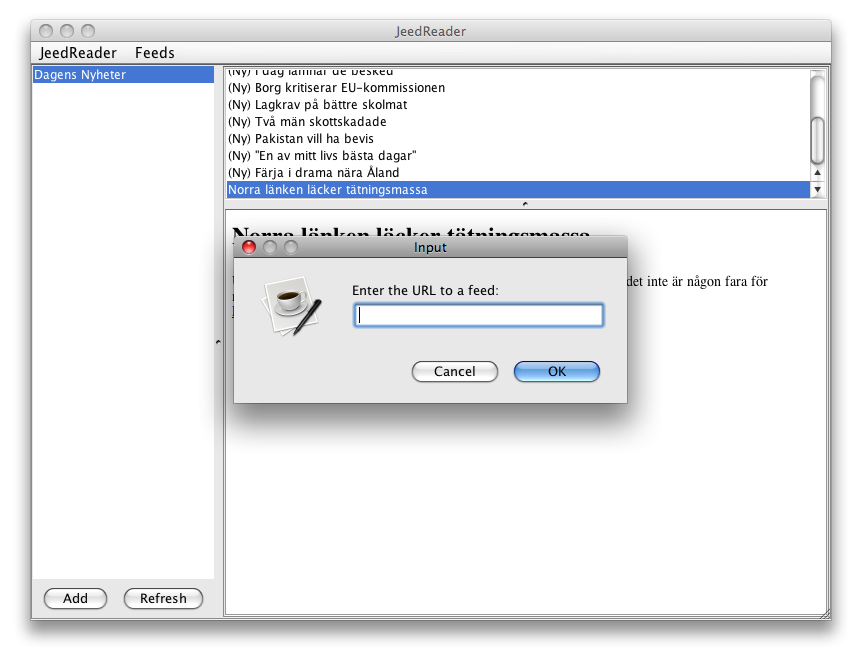
\includegraphics[width=110mm]{images/add-feed.png}
    \caption{Lägga till flöde.}
    \label{fig:add-feed}
  \end{center}
\end{figure}

Fyller användaren i en textsträng som inte uppfyller kraven för en
URL, kommer dialogruta i figur \ref{fig:malformed-url} visas. Det
finns även andra typer av felmeddelanden som återspeglar felaktiga
flöden. Exempel på detta är om användaren fyller i en URL som inte
pekar på ett RSS flöde av version 2.0, då visas felmeddelande:

\verb!Rss versions other than 2.0 is not supported.!.

Pekar inskriven URL inte på någon resurs alls fås felmeddelandet:

\verb!Resource not found.!

Detta är även fallet om det inte finns någon anslutning till
Internet.

\begin{figure}[!hbp]
  \begin{center}
    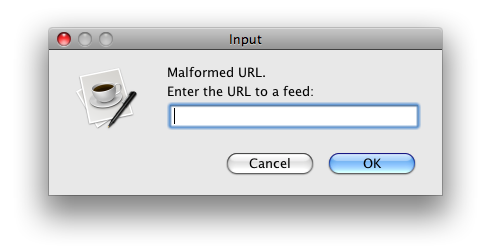
\includegraphics[width=110mm]{images/malformed-url.png}
    \caption{Felformaterad URL.}
    \label{fig:malformed-url}
  \end{center}
\end{figure}

\subsection{Läsa artikel}
För att läsa en artikel markeras ett flöde till vänster i
gränssnittet, sedan markeras en artikel i listan som dyker upp till
höger om flödena. Då visas artikelns innehåll i fältet under
artiklarna, se figur \ref{fig:read-item-out}.

\begin{figure}[!hbp]
  \begin{center}
    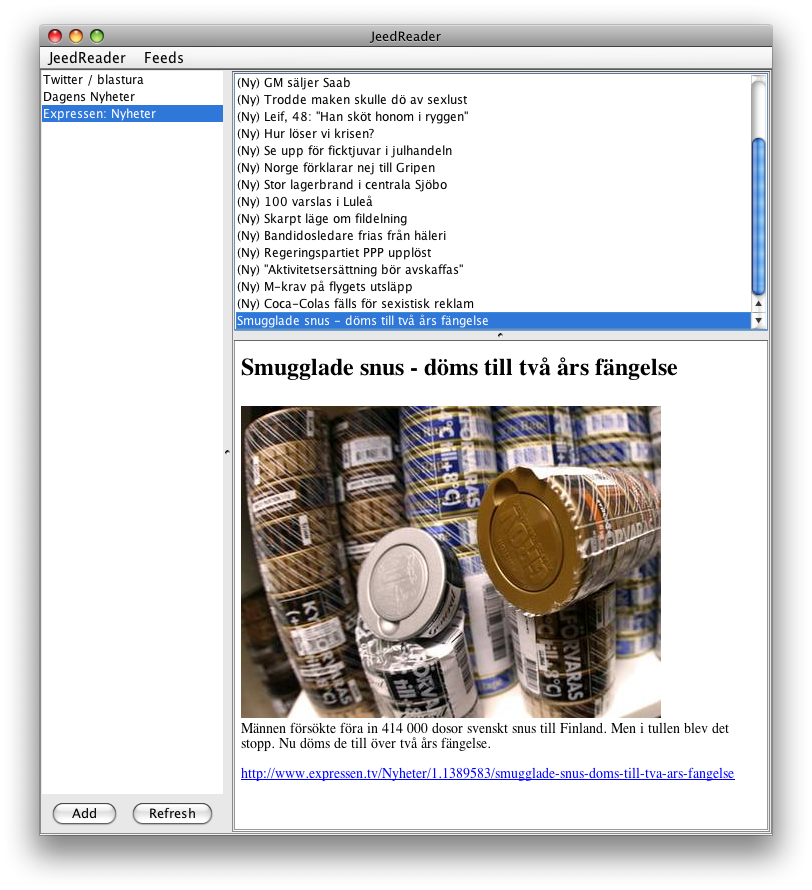
\includegraphics[width=110mm]{images/read-item-out.png}
    \caption{Läsa artikel.}
    \label{fig:read-item-out}
  \end{center}
\end{figure}

Innehållet i en artikel visas som \textit{html} vilket innebär att
bilder kommer att visas. En länk som hänvisar till artikelns ursprung
visas även men i nuläget händer ingenting om användaren klickar på
länken. Dock går det ju alltid att klippa ut och klistra in i en
webbläsare.

\subsection{Uppdatering av flöden}
Här följer ett scenario som visar på en uppdatering där en ny artikel
tillagts i ett flödes ursprungliga resurs. I
RSSxml~\ref{verb:1-test-xml} visas ett RSS-flödet innan uppdatering
sker. Läggs detta flöde till i programmet ser gränssnittet ut enligt
figur~\ref{fig:update-test1-out}.

\begin{program}
\begin{footnotesize}
\begin{verbatim}
<?xml version="1.0" encoding="iso-8859-1"?>
<rss version="2.0">
  <channel>
    <title>Localhost test</title>
    <link>http://localhost/~anton/test.xml</link>
    <description>Test kanal</description>

    <item>
      <title>Test titel</title>
      <link>http://localhost/~anton/</link>
      <description>Test beskrivning</description>
    </item>
  </channel>
</rss>
\end{verbatim}
\end{footnotesize}
\caption{Flöde innan uppdatering.}
\label{verb:1-test-xml}
\end{program}

\begin{figure}[!hbp]
  \begin{center}
    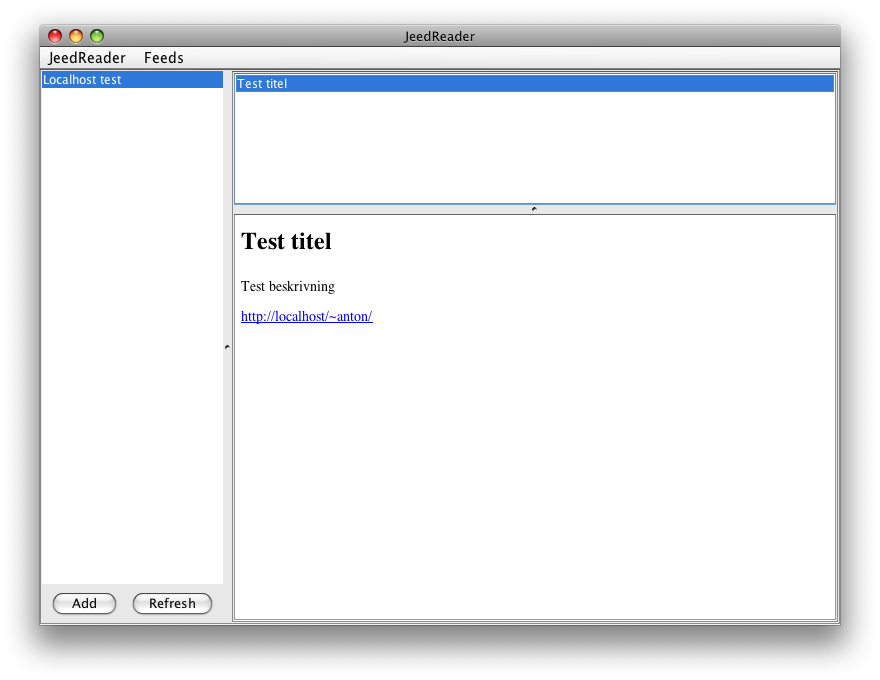
\includegraphics[width=110mm]{images/update-test1-out.png}
    \caption{Före uppdatering.}
    \label{fig:update-test1-out}
  \end{center}
\end{figure}

Läggs en ny artikel (element av typen \verb!<item/>!) till i flödet
och användaren uppdaterar flödet kommer gränssnittet att se ut enligt
figur~\ref{fig:update-test2-out}. Flödets utseende visas i
RSSxml~\ref{verb:2-test-xml}:

\begin{figure}[!hbp]
  \begin{center}
    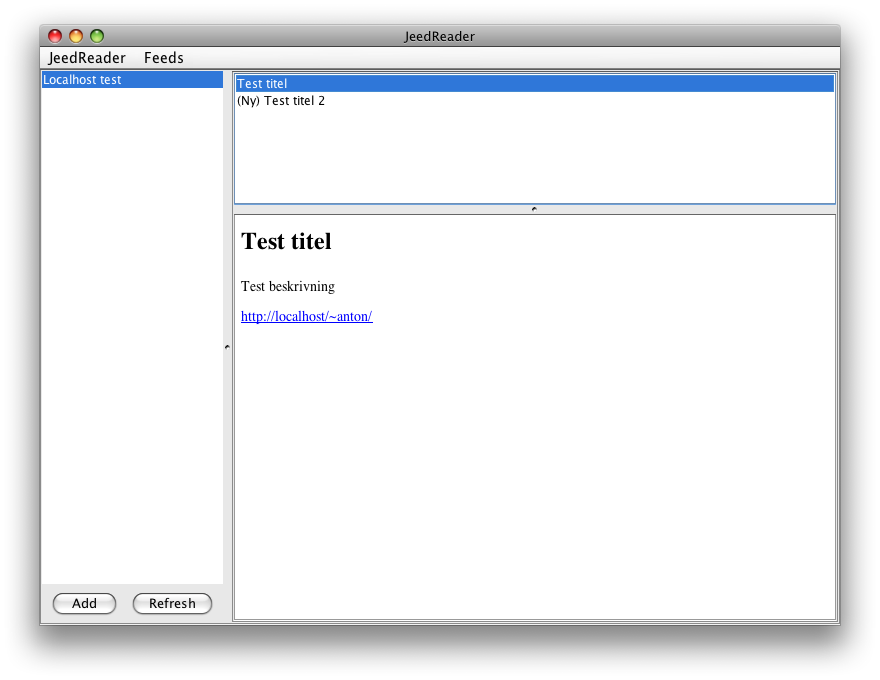
\includegraphics[width=110mm]{images/update-test2-out.png}
    \caption{Efter uppdatering.}
    \label{fig:update-test2-out}
  \end{center}
\end{figure}

\begin{program}
\begin{footnotesize}
\begin{verbatim}
<?xml version="1.0" encoding="iso-8859-1"?>
<rss version="2.0">
  <channel>
    <title>Localhost test</title>
    <link>http://localhost/~anton/test.xml</link>
    <description>Test kanal</description>

    <item>
      <title>Test titel</title>
      <link>http://localhost/~anton/</link>
      <description>Test beskrivning</description>
    </item>

    <item>
      <title>Test titel 2</title>
      <link>http://localhost/~anton/</link>
      <description>Test beskrivning</description>
    </item>
  </channel>
</rss>
\end{verbatim}
\end{footnotesize}
\caption{Flöde efter uppdatering.}
\label{verb:2-test-xml}
\end{program}

Konfigurationsfilen som programmet har sparat undan för att
handlingarna användaren har utfört har för detta flöde nu utseendet
som visas i RSSxml~\ref{verb:jss-xml}. Detta flöde är sparat till
hårddisken i mappen \textit{config} i samma mapp som klassfilerna
ligger. Filnamnet är:

\verb!http---localhost--anton-test-xml-feed.xml!p

\begin{program}
\begin{footnotesize}
\begin{verbatim}
<?xml version="1.0" encoding="UTF-8"?>
<jss version="2.0" feedLink="http://localhost/~anton/test.xml">
  <channel>
    <title>Localhost test</title>
    <link>http://localhost/~anton/test.xml</link>
    <description>Test kanal</description>
    <item isRead="true">
      <title>Test titel</title>
      <description>Test beskrivning</description>
      <link>http://localhost/~anton/</link>
    </item>
    <item isRead="false">
      <title>Test titel 2</title>
      <description>Test beskrivning</description>
      <link>http://localhost/~anton/</link>
    </item>
  </channel>
</jss>
\end{verbatim}
\end{footnotesize}
\caption{Flöde som sparas av programmet.}
\label{verb:jss-xml}
\end{program}

\section{Diskussion}\label{Diskussion}
% Hur fungerade det att följa en kodkonvention? Vilka var fördelarna
% respektive nackdelarna?
Laboration har varit intressant och givande, dock var det väldigt
svårt att få kläm på både trådar och grafiskt gränssnitt samtidigt då
detta bortsett från laboration 1 var första försöket på att
implementera ett liknande program.

Det skulle vara bra med mer belysande exempel under föreläsningarna
eller som utdelad kod, där man får givet ett klassdiagram och bra
design mönster har följts. Det svåra är nästan alltid att komma på ett
bra sätt att designa ett program. Har man inte gjort liknande program
förut är sannolikheten att man börjar i fel ände stor.

Min implementation fick en del klasser där jag enbart implementerade
statiska metoder. Hur fungerar dessa jämfört vanliga klasser och
metoder, exempelvis skulle metoderna FeedParsers kunna vara statiska,
de ändrar enbart värden som de fått in som parametrar. Dessa klasser
har jag deklarerat som \textit{final}, detta ska ge en snabbare
implementation enligt:\\
\verb!http://www.glenmccl.com/perfj_025.htm!\\


\newpage
\appendix
\pagenumbering{arabic}
\section{Källkod}\label{Kallkod}
% Källkoden ska finnas tillgänglig i er hemkatalog
% ~/edu/apjava/lab1/. Bifoga även utskriven källkod.
Härefter följer utskrifter från källkoden till denna laboration.

\subsection{Feed.java}\label{Feed.java}
\begin{footnotesize}
  \verbatiminput{../src/Feed.java}
\end{footnotesize}

\newpage
\subsection{FeedItem.java}\label{FeedItem.java}
\begin{footnotesize}
  \verbatiminput{../src/FeedItem.java}
\end{footnotesize}

\newpage
\subsection{FeedOutputter.java}\label{FeedOutputter.java}
\begin{footnotesize}
  \verbatiminput{../src/FeedOutputter.java}
\end{footnotesize}

\newpage
\subsection{FeedParser.java}\label{FeedParser.java}
\begin{footnotesize}
  \verbatiminput{../src/FeedParser.java}
\end{footnotesize}

\newpage
\subsection{FeedUtil.java}\label{FeedUtil.java}
\begin{footnotesize}
  \verbatiminput{../src/FeedUtil.java}
\end{footnotesize}

\newpage
\subsection{JeedConfigParser.java}\label{JeedConfigParser.java}
\begin{footnotesize}
  \verbatiminput{../src/JeedConfigParser.java}
\end{footnotesize}

\newpage
\subsection{JeedConfigWriter.java}\label{JeedConfigWriter.java}
\begin{footnotesize}
  \verbatiminput{../src/JeedConfigWriter.java}
\end{footnotesize}

\newpage
\subsection{JeedModel.java}\label{JeedModel.java}
\begin{footnotesize}
  \verbatiminput{../src/JeedModel.java}
\end{footnotesize}

\newpage
\subsection{JeedReader.java}\label{JeedReader.java}
\begin{footnotesize}
  \verbatiminput{../src/JeedReader.java}
\end{footnotesize}

\newpage
\subsection{JeedView.java}\label{JeedView.java}
\begin{footnotesize}
  \verbatiminput{../src/JeedView.java}
\end{footnotesize}

\newpage
\subsection{RssFeed.java}\label{RssFeed.java}
\begin{footnotesize}
  \verbatiminput{../src/RssFeed.java}
\end{footnotesize}

\newpage
\subsection{RssItem.java}\label{RssItem.java}
\begin{footnotesize}
  \verbatiminput{../src/RssItem.java}
\end{footnotesize}

\newpage
\subsection{RssParser.java}\label{RssParser.java}
\begin{footnotesize}
  \verbatiminput{../src/RssParser.java}
\end{footnotesize}
  
\end{document}